\documentclass[conference, 10pt, final]{IEEEtran}

\usepackage{cite}
\usepackage[cmex10]{amsmath}
\usepackage{amssymb}
\usepackage[pdftex]{graphicx}
\usepackage{algorithmic}
\usepackage{array}
\usepackage[caption=false,font=footnotesize]{subfig}
\usepackage{stfloats}
\usepackage{url}


\begin{document} 

\title{Improved Hierarchical Clustering Through Nesting}


\author{\IEEEauthorblockN{Alice Paul, Calvin Wylie, and David Lingenbrink}
\IEEEauthorblockA{Operations Research and Information Engineering, Cornell University, Ithaca, NY.  \\
Email: \{ ajp336, cjw278, dal299 \} @cornell.edu}}


\maketitle

\begin{abstract}
[TODO]
Hierarchical clustering organizes large data into smaller, more informative groups and offers a global view of the data structure by producing a hierarchy of clusters starting from individual data points and merging towards the cluster of all data. Typically, hierarchical clustering is done by greedily either merging or dividing clusters, called agglomerative and divisive clustering, respectively. Lin et al.~\cite{Lin} proposed a nesting framework that produces a hierarchal clustering from partitional clusterings for every possible number of clusters. This algorithm was introduced as an approximation algorithm for the hierarchical $k$-median problem and guarantees the resulting hierarchical layers are a limited distance from the original partitional clusters. However, this algorithm has not been previously placed in a clustering context. We test this algorithm using various methods for producing the partitional clusterings against the traditional hierarchical clustering methods and show both the approximation ratio and FScore measure improve significantly. We also propose a heuristic for this nesting framework which improves the run time and only suffers a slight decrease in approximation and FScore.
\end{abstract}


\section{Introduction and Notation}
Clustering algorithms date back more than 50 years, and there have been many variations introduced since \cite{Jain}.  The two main branches of clustering are partitional (or flat) and hierarchical. In partitional clustering, we often specify a number $k$ and pairwise distances between the data points, representing a measure of dissimilarity such as Euclidean distance. A clustering algorithm thus partitions the data into $k$ disjoint sets where the sets represent relatively similar data. For hierarchical clustering, we are interested in finding a nested tree of partitions. This offers the user a global view of the data and allows the user to choose a ``natural'' level of clustering \cite{ESL}.  Examples of both partitional and hierarchical clustering are given in Fig.~\ref{fig_part}-\ref{fig_hier}.

One common objective function for partitional clustering is to minimize the sum of distances from each point to the median point of its cluster, called $k$-median or $k$-medoids clustering. More specifically, suppose we are given a set $X$ and a distance (dissimilarity) metric $d(i,j)$ for all $i,j \in X$. The goal is to find a set of centers $S \subseteq X$ such that $|S| \leq k$ so as to minimize 
\[ f(S) = \sum_{ i\in X} \min_{j \in S} d(i,j). \]
The clustering is obtained from the set of centers $S$ by assigning each data point to its nearest center.  An $\alpha$-approximation algorithm for this problem produces a set $S$ in polynomial time such that $f(S) \leq \alpha \cdot f(O)$ for all $O \subseteq X$ with $|O| = k$. 

\begin{figure*}[!]
\centerline{\subfloat[Partitional Clustering]{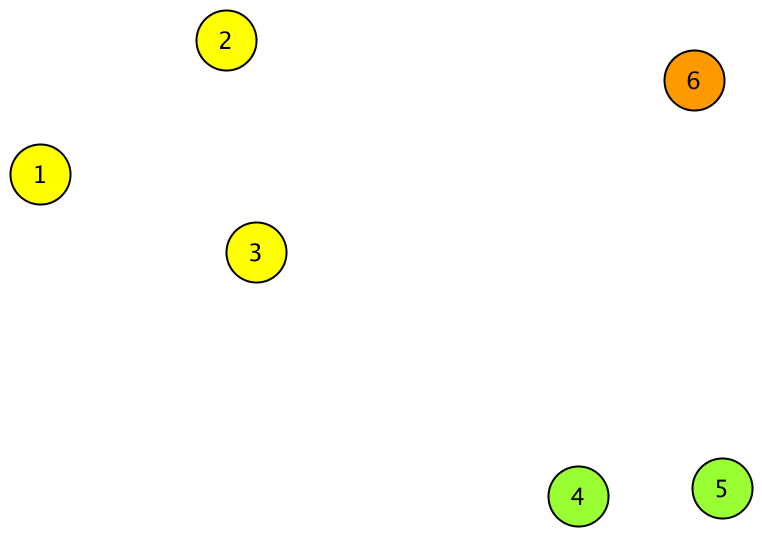
\includegraphics[width =1.75in]{partitional_clustering}
\label{fig_part}}
\hfil
\subfloat[Hierarchical Clustering]{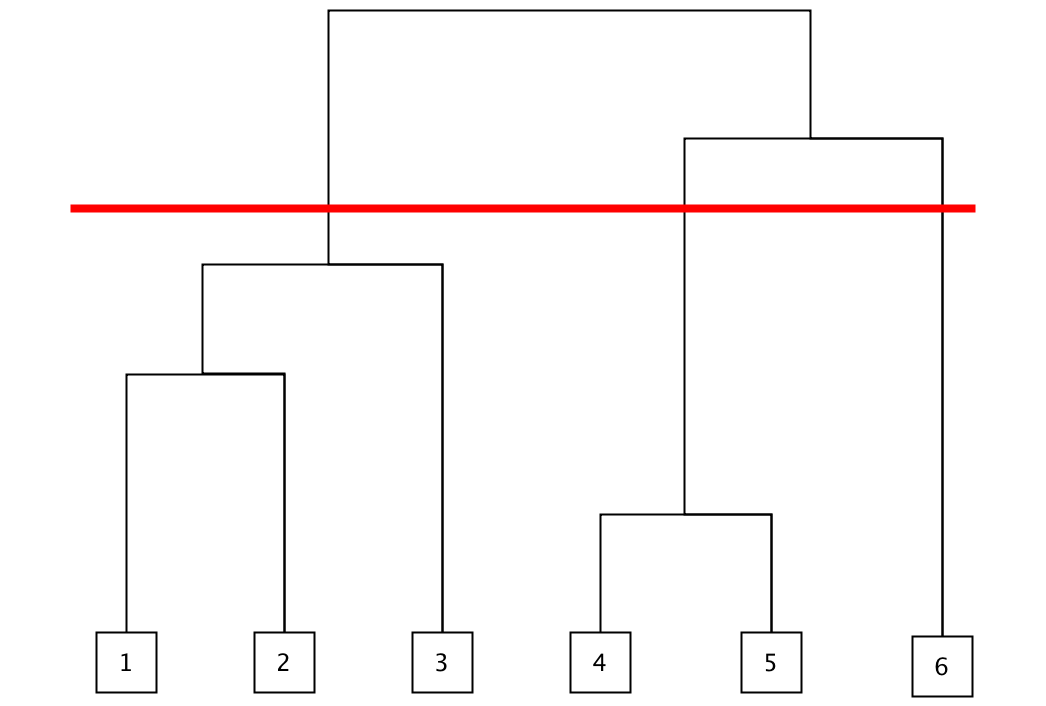
\includegraphics[width=2.5in]{hier_clustering}
\label{fig_hier}}}
\caption{A partitional clustering for $k=3$, where the colors represent the different partitions, and a dendrogram representation of a hierarchical clustering of the data, where edges represent mergeing of clusters.  Note the clustering on the third level (represented by the red line) corresponds to the partitional clustering on the left.}
\end{figure*}

This objective function can then be extended to the hierarchical $k$-median problem. Suppose we represent a solution to the $k$-median problem as a pair $(S, a)$ where $S \subseteq X$ such that $|S| \leq k$ and $a$ is an assignment function that maps each $i \in X$ to a center in $S$. Then, for any $i \in S$, $a^{-1}(i)$ is the cluster centered at $i$. We define $f(S,a) := \sum_{i \in X} d(i, a(i))$. Note this is the same objective function as above, except the assignment is given rather than implied.

Given solution pairs $(S_1, a_1)$ and $(S_2, a_2)$, we say that $(S_1, a_1)$ is \emph{nested} in $(S_2, a_2)$ (denoted $(S_1, a_1) \subseteq (S_2, a_2)$) if the following conditions hold:
\begin{enumerate}[\IEEEsetlabelwidth{3)}]
	\item $S_1 \subset S_2$, 
	\item $\forall  j \in X$, if $a_2(j) \in S_1$, then $a_1(j) = a_2(j)$, 
	\item $\forall j, k \in X$, if $a_2(j) = a_2(k)$, then $a_1(j) = a_1(k)$.
\end{enumerate}
A solution to the hierarchical $k$-median problem is a nested chain of solutions, and the hierarchical clustering it generates is found by looking at the clusters given by each $(S_i, a_i)$. An example is given in Fig.~\ref{fig_chain1}-\ref{fig_chain4}. 

We would like a nested hierachical solution to stay close to the optimal $k$-median solutions when looking at any level of the hierarchy. An $\alpha$-approximation algorithm for this problem generates a nested chain of solutions in polynomial time such that for all $k = 1, \ldots, |X|$ there exists $(S_i, a_i)$ in the chain such that $|S_i| \leq k$ and $f(S_i, a_i) \leq \alpha \cdot f(O)$ for all $O \subseteq X$ with $|O| = k$.

\begin{figure*}[b]
\centering
\subfloat[$(S_1, a_1)$]{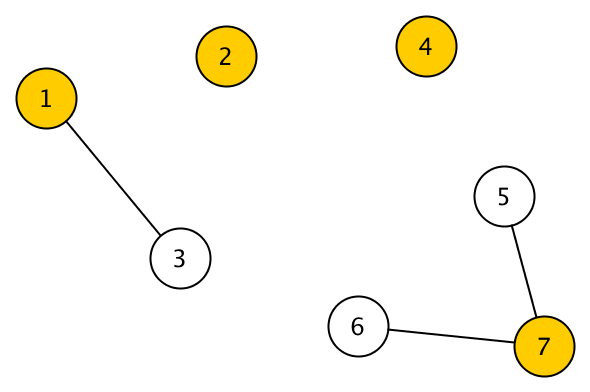
\includegraphics[width =1.75in]{chain1}
\label{fig_chain1}} \hspace{15mm}
\subfloat[$(S_2, a_2)$]{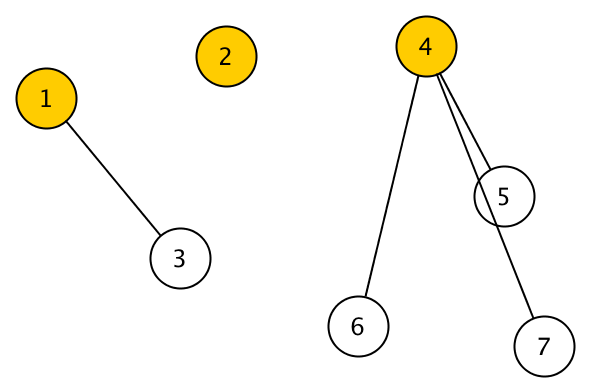
\includegraphics[width=1.75in]{chain2}
\label{fig_chain2}} \\
\subfloat[$(S_3, a_3)$]{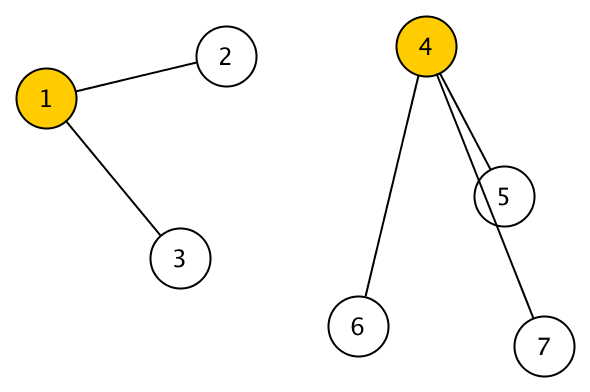
\includegraphics[width=1.75in]{chain3}
\label{fig_chain3}}  \hspace{15mm}
\subfloat[$(S_4, a_4)$]{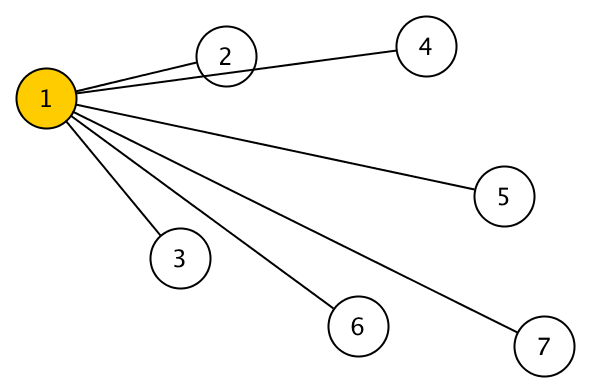
\includegraphics[width=1.75in]{chain4}
\label{fig_chain4}}
\caption{An example of a nested chain of solutions. $S_i$ is indicated by the colored nodes and $a_i$ by the edges. The clusters on that level are given by the connected components. Note that $S_{i-1}$ is a subset of $S_i$ and the assignments stay consistent. }
\label{fig_sim}
\end{figure*}

While some partitional clustering methods use the $k$-median objective function to inform their decisions, popular methods for hierarchical clustering do not and instead rely on greedy algorithms which have no guarantee on the solution produced with respect to the objective function but are typically fast and easy to implement. This paper looks at how using this objective function can vastly improve the hierarchical clusterings produced. 
In particular, we show how an approximation framework for this problem, which takes in partitional clusterings for all values of $k$, compares in practice to some of the most widely used clustering algorithms, both in the quality of the solution and in computation time. The algorithms we use to produce these partitional clusterings include both approximation algorithms for the $k$-median problem, which offer an overall approximation guarantee for the hierarchical $k$-median problem, and some heuristic algorithms that have been shown to perform well in practice. 

\section{Literature Review}

\subsection{Partitional Clustering}
Arguably the most common partitional clustering method is $k$-means, which chooses $k$ cluster centers in space so as to minimize the sum of squared distances from each point to its nearest cluster center \cite{Jain}.  $k$-means is usually solved using Lloyd's algorithm (also referred to simply as the $k$-means algorithm), which iteratively greedily updates the centers of each cluster (assigning points to the nearest center) until the solution becomes stable \cite{Jain}. Lloyd's algorithm is only guaranteed to reach a locally optimum solution and can be very sensitive to outliers and the initial points chosen \cite{Kanungo}.

The $k$-median objective function removes some worst-case behavior of $k$-means by restricting the cluster centers to be data points.  Two common algorithms for this problem are partition around medoids (PAM), and $k$-medoids. PAM is a local seach algorithm which starts with $k$ randomly chosen data points as centers, and looks to swap one of the centers with another data point to improve the objective value. This repeats until no more improving swaps exist \cite{ESL}. The generalization of this algorithm which considers swaps of size $\leq p$ is a $(3 + \frac{2}{p})$-approximation algorithm \cite{Arya}.
$k$-medoids, which is more computationally efficient than PAM \cite{Park}, is a variation on Lloyd's $k$-means algorithm.  Starting with randomly chosen centers, we assign each data point to its nearest center, and then update the center within each cluster \cite{Park}. The algorithm repeats this until the solution becomes stable.

The $k$-median problem is also a fundamental problem in approximation algorithms, where it is often presented in the context of opening service centers or factories to serve clients. However, these algorithms are often not implemented for clustering despite their improved guarantees on the solution. The best known approximation algorithm for this problem has an approximation guarantee of 2.592 and is produced using linear programming \cite{Wu}. A simpler LP rounding algorithm by Charikar and Li has a slightly worse guarantee of 3.25 but is easier to implement in practice \cite{Charikar}. 

\subsection{Hierarchical Clustering}
The most common method for hierarchical clustering is agglomerative clustering. The agglomerative clustering procedure starts with each data point in its own cluster, and recursively merges the two nearest clusters to form the next clustering level in the hierarchy, repeating until the entire data set is a single cluster.  There are several choices on how to measure distance in order to choose the nearest clusters to merge. Single linkage (also called nearest neighbor) defines the distance between two clusters to be the minimum pairwise distance between the data points in each cluster.  Complete linkage clustering instead defines the distance to be the largest pairwise distance. A method between these two extremes is group average linkage which looks at the average pairwise distance between clusters. This strikes a balance between the closeness and compactness of the two techniques above and gives more reasonable results in practice \cite{ESL}. Lastly, there is Ward's method which chooses the two clusters to merge so as to minimize the sum of each cluster's variance \cite{Ward}.

Approximation algorithms for hierarchical clustering have also been studied, where we aim to identify a hierarchy of clusters so as to minimize the ratio of the objective value on every level in the hierarchy of size $k$ to the optimal objective value of the partitional clustering problem with $k$ clusters. Note that it may not always be possible to find a solution with approximation ratio 1. The hierarchical $k$-median problem was originally introduced by Plaxton who gave a 238.88 approximation algorithm \cite{Plaxton}. This was improved by Lin et al.~\cite{Lin} who gave an incremental approximation algorithm framework. Their approach relies on a black box $k$-median solver and then uses these solutions for $k=1, \ldots, n$ to greedily construct a hierarchical clustering that increases the objective value by at most a factor of $20.71$ (or $10.03$ when randomized) at each level. Using the local $p$-swap $(3+\frac{2}{p})$-approximation algorithm mentioned above as the black-box $k$-median solver performed well in experiments on hierarchical $k$-median test problems \cite{Nagarajan}. While the authors tested the variants of this algorithm for different $k$-median approximation algorithms, it has not been tested against traditional clustering algorithms or on any labeled data sets. 

Several algorithms have been built upon agglomerative clustering that we choose not to compare with our proposed algorithms. Divisive clustering, similar to agglomerative, starts with the data in one cluster and repeatedly splits a cluster on each level. This method has not been studied nearly as much as agglomerative clustering \cite{ESL} but has had relative success in classifying document datasets \cite{Zhao}.  Algorithms such as the CURE, ROCK, and Chameleon \cite{Guha_CURE, Guha_ROCK, Karypis} incorporate non-spherical cluster shapes and cluster density, but do not relate as much to the above approximation algorithm in their objective. We also choose not to compare our algorithms with Bayesian hierarchical methods since these methods require many more parameters and add additional prior information that our algorithms do not use. 

\section{Proposed Algorithms}

\subsection{Hierarchical Algorithm} 

Recall the hierarchical $k$-median problem: given a set $X$ and a distance metric $d(i,j)$ for all $i,j \in X$, we represent a solution to the $k$-median problem as a pair $(S, a)$ where $S \subseteq X$ such that $|S| \leq k$ and $a$ is an assignment function that maps each $i \in X$ to a center in $S$.
 A solution to the hierarchical $k$-median problem is a chain of nested solutions $(S_1, a_1) \subseteq (S_2, a_2) \subseteq \ldots \subseteq (S_n, a_n)$. However, we want this solution to stay close to the optimal $k$-median solutions when looking at any level of the hierarchy.  
Consider any $k$-median algorithm $\mathcal{A}$. After running $\mathcal{A}$ for all potential values of $k$, Lin et al.~\cite{Lin} introduce an augmentation step that nests these clusterings into the hierarchical framework and only increase costs by a bounded factor. 

First, set $\beta = 3+\sqrt{3}$, and $\beta_0 = 1$ (for the randomized algorithm we instead let $\beta = 6.355$ and set $\beta_0 = \beta^X$, where $X$ is drawn uniformly from $[0,1]$). Let $V_i$ be the solutions generated from running $\mathcal{A}$ for $k=n-i+1$ for $i=1, \ldots, n$. The cost of these solutions is determined by assigning each point to the nearest cluster center and is scaled so that the minimum cost for $k<n$ is at least one. We then bucket these solutions by cost into buckets of the form $[0,0], (\beta_0, \beta_0 \beta], (\beta_0 \beta, \beta_0 \beta^2], \ldots $. 

From each non-empty bucket, pick the solution with the smallest number of cluster centers, and let these solutions be $\overline{V}_1, \overline{V}_2, \ldots \overline{V}_r$. We then inductively build our nested solutions: Set $S_1 = \overline{V}_1$ and $a_1$ to be the assignment that assigns each point to the nearest point in $S_1$. Given $(S_{i-1}, a_{i-1})$ and $\overline{V}_i$, we construct $S_i$ by  adding the nearest point $j \in S_{i-1}$ to $l$ for each $l \in \overline{V}_i$. Note that $|S_{i}| \leq |\overline{V}_i|$. 

\begin{figure*}[!t]
\centering
\subfloat[Nested solution $(S_{i-1}, a_{i-1})$ ]{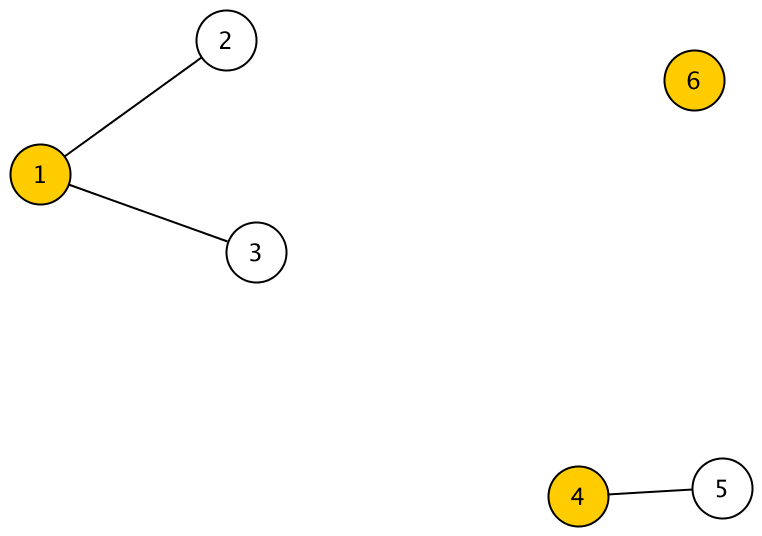
\includegraphics[width =1.75in]{Si-1}
\label{fig_Si-1}} \hspace{15mm}
\subfloat[Next set $\bar{V}_i$]{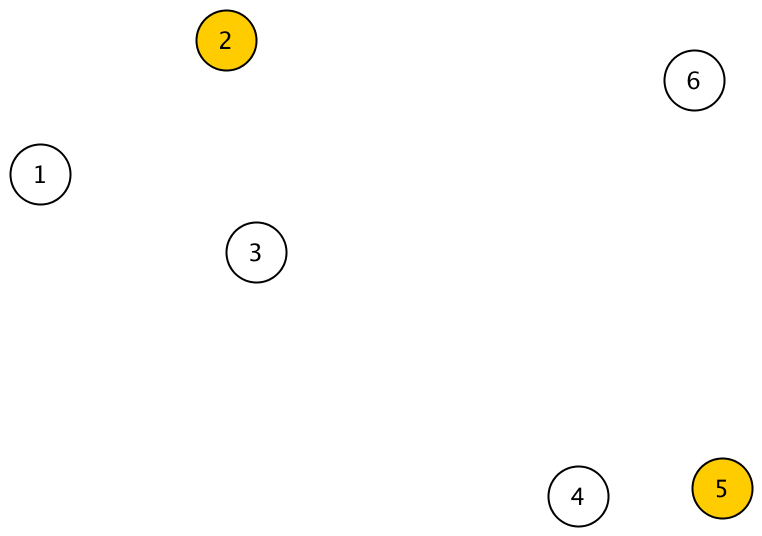
\includegraphics[width=1.75in]{Vi}
\label{fig_Vi}} \\
\subfloat[Next nested centers $S_i$]{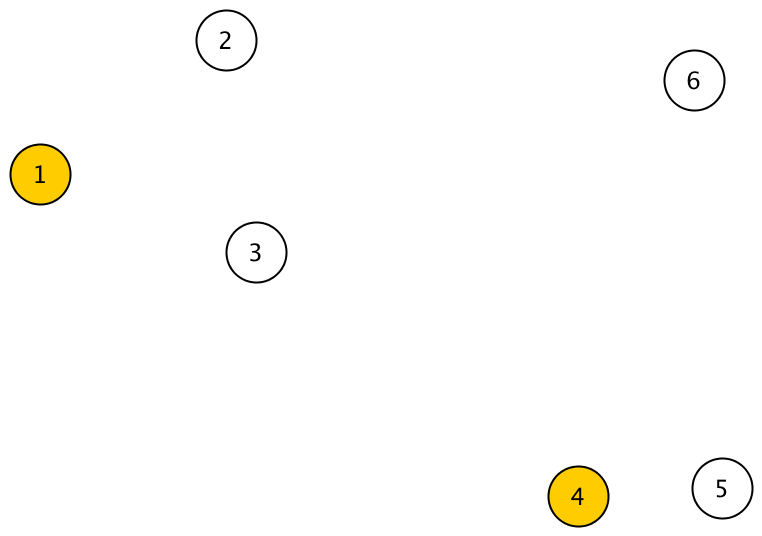
\includegraphics[width=1.75in]{Si}
\label{fig_Si}}  \hspace{15mm}
\subfloat[Next nested solution $(S_i, a_i)$]{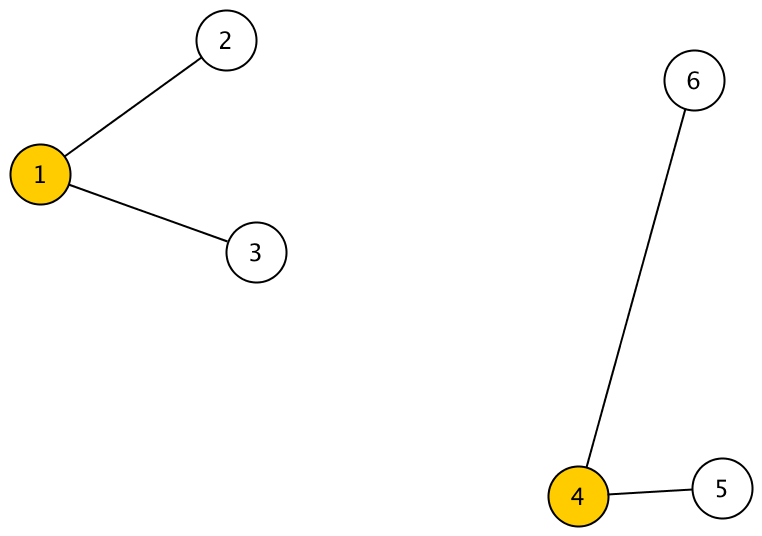
\includegraphics[width=1.75in]{Siai}
\label{fig_Siai}}
\caption{An example of nesting $\bar{V}_i$ with $(S_{i-1}, a_{i-1})$. Dark  nodes represent chosen centers and edges represent assignments to that center's cluster. }
\label{fig_sim}
\end{figure*}
% First, node 2 chooses node from 1 from $S_{i-1}$ as its nearest center and node 5 chooses node 4. Then, each cluster in $(S_{i-1}, a_{i-1})$ is assigned to the cheapest (lowest sum of distances) center.

We then need to define an assignment $a_i$. For each $j \in X$ such that $a_{i-1}(j) \in S_{i}$, we set $a_i(j) = a_{i-1}(j)$. Otherwise, we set $a_i(j)$ to be the point $i \in S_i$ such that assigning all points in $a_{i-1}^{-1}(j)$ (i.e. all points in $j$'s cluster in $S_{i-1}$) would have minimum cost. Using this assignment, $(a_i, S_i)$ is nested in $(a_{i-1}, S_{i-1})$. An example of this nesting is given in Fig.~\ref{fig_Si-1}-\ref{fig_Siai}.

We continue this nesting until $|S_i| = 1$, reaching the top level of the hierarchy where all data points are in the same cluster. After forming this hierarchical clustering, for any $k \in 1, \ldots, n$ \cite{Lin} guarantees that the cost of $S_i$ is at most $20.71$ times the cost of $V_k$ where $|S_{i-1}| \geq |V_k| \geq |S_{i}|$ (in the randomized case the expected cost of $S_i$ is at most $10.03$ times the cost of $V_k$).


\subsection{Partitional Clustering Algorithms}
Since the described nesting framework allows us to choose the partitional clustering algorithm $\mathcal{A}$, the choice of this algorithm is critical. PAM has the added benefit of being a 5-approximation algorithm for the partitional $k$-median problem, which yields to an overall approximation ratio of $20.71 \cdot 5 = 103.55$ for the hierarchical $k$-median problem ($10.03 \cdot 5 = 50.15$ randomized). We looked at increasing the size of the local swaps in PAM to improve the approximation ratio but found that the approximation ratio of constructed solutions for given values of $k$ did not significantly improve while the computation time increased greatly. 

We also consider three linear programming based algorithms, one of which has an approximation guarantee. We first present the integer programming formulation for the $k$-median problem. Suppose we have a set $X$. Let for all $i \in X$, $s_i \in \{0,1\}$ be variables representing whether or not we want to make $i$ a center. We also create variables $a_{i,j} \in \{0, 1\}$ which represent whether or not we assign $i \in X$ to the cluster with center $j \in X$. Given this set and assignment, and distance metric $d$, the $k$-median objective function is 
\begin{equation}
\sum_{i \in X} \sum_{j \in X} a_{i,j} d(i,j), 
\end{equation}
which we want to minimize. However, we are restricted to choosing at most $k$ centers, every point must be assigned to a single cluster center, and we can only assign a point to another point that has actually been chosen as a center. These restrictions are represented by the following constraints, respectively:
\begin{eqnarray}
\sum_{i \in X} s_i   \leq k & ,\\
\sum_{j \in X} a_{i,j}  = 1 & \forall i \in X, \\
a_{i,j}   \leq s_j & \forall i, j \in X.
\end{eqnarray}
Therefore, solving the following integer program would directly find the optimal set of centers and assignment for the $k$-median problem.
\begin{eqnarray}
\text{Min } & \sum_{i \in X} \sum_{j \in X} a_{i,j} d(i,j) \\
\text{s.t. } & \sum_{i \in X} s_i   \leq k  \\
& \sum_{j \in X} a_{i,j}  = 1 \quad \forall i \in X \\
& a_{i,j}   \leq s_j \quad \forall i, j \in X \\
& s_i \in \{0,1\} \quad \forall i \in X \\
& a_{i,j} \in \{0,1\} \quad \forall i, j \in X.
\end{eqnarray}
Relaxing the constraints to $s_i \in [0,1]$ for all $i \in X$ and $a_{i,j} \in [0,1]$ for all $i,j \in X$ yields the linear programming (LP) relaxation for the $k$-median problem, which can be solved in polynomial time.

Interestingly, the solution to the LP relaxation is often integer valued \cite{Nagarajan}. In light of this, we propose two LP-based clustering algorithms that both first solve the LP relaxation.  The first proposed algorithm constructs the set of centers $S$ by taking the points in $X$ with the $k$ highest $s_i$ values.  The second constructs $S$ by choosing $i$ to be in $S$ with probability $s_i$, sampling for each $i \in X$ until $k$ centers are chosen. We refer to these algorithms as LP-greedy and LP-rand, respectively.

Charikar and Li \cite{Charikar} introduce a 3.25-approximation algorithm that uses LP relaxation solution to smartly construct a set of centers. We refer to this algorithm as LP-Charikar. We chose to implement this LP algorithm, rather than the LP-based approximation algorithm with best approximation ratio, because LP-Charikar is simpler to implement, and expected to have a lower running time.  

[MAYBE CUT THE ALGORITHM DESCRIPTION AND SAY TO REFER TO THE ORIGINAL PAPER?]
The algorithm first chooses a subset of data points $C \subseteq X$ to represent the demand. For each data point $i$, let $d_{av}(i) = \sum_{j \in X : a_{i,j} > 0} s_j \cdot d(i,j)$. We start with $C = \emptyset$. At each step, we choose a point $j \in X$ to add to $C$, and all points $j'$ such that $d(j,j') \leq 4 d_{av}(j') $ are removed from $X$. This is continued until $X$ is empty. 

$C$ now represents data points that are relatively far apart. These points then choose a bundle of points $U_j$ that represent potential centers they would like to be assigned to. In particular, for each point $j \in C$, we look at all points $i \in X$ such that $0 < d(i,j) < 1.5 R_j$, where $R_j$ is half the distance from $j$ to its nearest point in $C$, and bundle these points into $U_j$ (if a point is in multiple bundles, choose one arbitrarily). Now these bundles of points have a sum of $s_i$ values of at least one half. For each $U_j$, we define the volume of $U_j$ to be $\mathrm{vol}(U_j) = \sum_{i \in U_j} s_i$. Lastly, these bundles are matched together greedily by distance. 

Now that the algorithm has grouped and matched together points so that the volume is at least 1, the algorithm starts choosing points from these various groups through sampling. Here, opening $U_j$ refers to selecting a point $i \in U_j$ with probabilities proportional to the $s_i$ values and adding that point to $S$. 
\begin{enumerate}[\IEEEsetlabelwidth{3)}]
\item For each matched $U_j$ and $U_{j'}$, the algorithm opens $U_j$ with probability $1-\mathrm{vol}(U_{j'})$, opens $U_{j'}$ with probability $1- \mathrm{vol}(U_j)$, and opens both $U_{j}$ and $U_{j'}$ with probability $\mathrm{vol}(U_j) + \mathrm{vol}(U_{j'}) -1$. 
\item For any unmatched $U_j$, it is opened with probability $\mathrm{vol}(U_j)$.
\item For any $i$ not in any $U_j$ such that $s_i > 0$, add $i$ to $S$ with probability $s_i$. 
\end{enumerate}
This sampling process returns a set of centers of size $k$  in expectation and produces a set $S$ such that $\mathbb{E}[f(S)] \leq 3.25 \cdot f(O)$ for all $O \subseteq X$ such that $|O| = k$. For our purposes, we sample until we obtain a solution with exactly $k$ centers. 

\section{Implementation and Results}

\subsection{Implementation Specifics}

All tests were conducted using Python 2.7.9 on a 64-bit Windows platform with a 4 core 3.4 Ghz Intel i7 processor and 16 GB physical memory. All code and the full computational results are available at \url{https://github.com/apaul29/Hierarchical-Code}.
We tested the algorithms on the following data sets:
\begin{LaTeXdescription}
\item[Gaussian] 27 synthetic $k$-center Gaussian data sets, generated in Python. In particular, Gauss\textunderscore d\textunderscore k\textunderscore e was generated by first choosing $k$ random centers in $[-1,1]^d$. Around each center, we then generated $(1000/k) \cdot \mathrm{Unif}[0,1]$ Gaussian points of which $e$ percent had standard deviation 0.25 (noisy) and $1-e$ percent had standard deviation $0.05$. 
\item[OR $p$-median Library] \cite{Beasley} From a collection of classic test data sets for approximation algorithms created by Beasley with 40 test sets of size $100, 200, \ldots, 900$ and varying values of $k$. This data is unlabeled.
\item[UCI Iris] \cite{Iris} Contains 4 attributes on 150 instances of flowers, each of with belongs to one of three species of iris.  One of the species is linearly separable from the others, but the other two are not.  One of the most used data sets in pattern recognition.
\item[UCI Soybean (Small)] \cite{Soybean} 47 instances, with 35 attributes data set of soybean disease from UCI.
\end{LaTeXdescription} 

\begin{table}[!t]
\caption{Some specifics about our datasets}
\label{table_specifics}
\centering
\begin{tabular}{ | l | l | l | l | l | }
\hline
 Dataset Name & Opt Obj & $k$ & $n$ & dim \\ \hline
Soybean & 113.805 & 4 & 47 & 35 \\ 
Iris & 98.214 & 3 & 150 & 4 \\ 
Gauss\_5\_5\_5 & 195.414 & 5 & 388 & 5 \\ 
Gauss\_5\_10\_5 & 270.066 & 10 & 544 & 5 \\ 
Gauss\_5\_50\_5 & 178.122 & 50 & 408 & 5 \\ 
Gaussian avg & 241.497 & 21.7 & 507 & 5 \\ 
pmed5 & 1355 & 33 & 100 & \  \\ 
pmed20 & 1789 & 133 & 400 & \  \\ 
pmed35 & 10400 & 5 & 800 & \  \\ 
$p$-median avg & 5535.3 & 45.9 & 460 & \  \\ \hline
 \end{tabular}
\end{table}

\subsection{Partitional Algorithms}
For $k$-median algorithms, we implemented $k$-medoids, PAM, LP-greedy, LP-rand, and LP-Charikar in Python, using Gurobi 6.0.3 to solve the linear programs. 
To avoid cycling, we limited the number of iterations in $k$-medoids to 1000. For PAM, we also limit the number of swaps to achieve a reasonable runtime. Instead of searching over all potential swaps, we sample at most $n$ potential swaps. We also ensure that some minimum progress is achieved by ensuring the algorithm decreases in objective by at least a factor of 0.9 in each iteration. At the end of PAM, we run 10 iterations of $k$-medoids to ensure the algorithm finds a local optimum. These choices were made by looking at the relative performance and computation time on random Gaussian data not included in the data sets described above.

Before implementing these data sets in the hierarchical framework, we compared them as partitional algorithms on the data above which had given values of $k$. For context, we also included the results from running $k$-means (implemented in the scikit-learn package in Python) and the extension of PAM called 2-swaps that also looks at local swaps of size 2 (which improves the $k$-median approximation ratio to 4 from 5). 

For each data set and each partitional clustering method, we recorded the approximation ratio (for the flat $k$-median objective function), computation time, and, where applicable, adjusted mutual information (AMI).  AMI is a measure which scores accuracy of predicted clusters compared to a true labeling by measuring the agreement of two assignments. The measure is normalized to reflect chance, so that a perfect labeling receives a score of 1 and an independent random labeling receives a score of 0 in expectation.  See \cite{Vinh} for further information.  Results are given in Tables~\ref{fig:flat_results_comp}-\ref{fig:flat_results_approx}  below with some results averaged due to space constraints. The results reported are average values across 10 trials.

\begin{table*}[!t]
\caption{Average Computation Time (sec) for Partitional Clustering Algorithms.}
\centering
\begin{tabular}{ | l | l | l | l | l | l | l | l|}
\hline
Dataset	&	k-means	&	k-medoids	&	PAM	&	2-swaps	&	LP-Charikar	&	LP-greedy	&	LP-rand	\\ \hline
Soybean	&	0.0151	&	0.0020	&	0.0159	&	0.0493	&	0.1180	&		&		\\
Iris	&	0.0129	&	0.0030	&	0.1018	&	0.2294	&	1.4644	&		&		\\
Gauss\_5\_5\_5	&	0.0249	&	0.0318	&	1.5058	&	2.3824	&	18.1701	&		&		\\
Gauss\_5\_10\_5	&	0.0540	&	0.1085	&	5.4071	&	9.4277	&	47.7316	&		&		\\
Gauss\_5\_50\_5	&	0.1371	&	0.3019	&	21.4457	&	39.6144	&	17.5115	&		&		\\
Gaussian avg	&	0.0730	&	0.1817	&	13.0214	&	18.6957	&	37.2315	&		&		\\
pmed5	&	N/A	&	0.0381	&	0.6223	&	0.7479	&	0.5357	&		&		\\
pmed20	&	N/A	&	1.7947	&	44.9791	&	68.2306	&	18.2055	&		&		\\
pmed35	&	N/A	&	0.1133	&	5.8814	&	9.2881	&	117.4038	&		&		\\
$p$-median avg	&	N/A	&	0.8072	&	40.3474	&	56.7595	&	46.1541	&		&		\\ \hline
\end{tabular}
\label{fig:flat_results_comp}
\end{table*}

\begin{table*}[!t]
\caption{Average AMI measure for Partitional Clustering Algorithms.}
\centering
\begin{tabular}{ | l | l | l | l | l | l | l | l| }
\hline
Dataset	&	k-means	&	k-medoids	&	PAM	&	2-swaps	&	LP-Charikar	&	LP-greedy	&	LP-rand	\\ \hline
Soybean	&	0.686	&	0.550	&	0.732	&	0.708	&	0.721	&		&		\\
Iris	&	0.748	&	0.690	&	0.760	&	0.757	&	0.647	&		&		\\
Gauss\_5\_5\_5	&	0.741	&	0.687	&	0.749	&	0.744	&	0.754	&		&		\\
Gauss\_5\_10\_5	&	0.783	&	0.677	&	0.725	&	0.737	&	0.729	&		&		\\
Gauss\_5\_50\_5	&	0.646	&	0.621	&	0.619	&	0.631	&	0.631	&		&		\\
Gaussian avg	&	0.777	&	9.112	&	0.761	&	0.761	&	0.767	&		&		\\ \hline
\end{tabular}
\label{fig:flat_results_AMI}
\end{table*}


\begin{table*}[!t]
\caption{Average Approximation Coefficients for Partitional Clustering Algorithms.}
\centering
\begin{tabular}{ | l | l | l | l | l | l| l|}
\hline
Dataset	&	k-medoids	&	PAM	&	2-swaps	&	LP-Charikar	&	LP-greedy	&	LP-rand	\\ \hline
Soybean	&	1.167	&	1.012	&	1.012	&	1.000	&		&		\\
Iris	&	1.081	&	1.004	&	1.004	&	0.873	&		&		\\
Gauss\_5\_5\_5	&	1.070	&	1.002	&	1.005	&	1.002	&		&		\\
Gauss\_5\_10\_5	&	1.080	&	1.011	&	1.009	&	1.020	&		&		\\
Gauss\_5\_50\_5	&	1.089	&	1.020	&	1.014	&	1.001	&		&		\\
Gaussian avg	&	1.064	&	1.009	&	1.008	&	1.004	&		&		\\
pmed5	&	1.373	&	1.026	&	1.033	&	1.000	&		&		\\
pmed20	&	1.501	&	1.032	&	1.027	&	1.000	&		&		\\
pmed35	&	1.083	&	1.005	&	1.007	&	1.027	&		&		\\
$p$-median avg	&	1.187	&	1.017	&	1.019	&	1.000	&		&		\\ \hline
\end{tabular}
\label{fig:flat_results_approx}
\end{table*}


[ADD FLAT RESULT ANAYLIS]

It is interesting to note that, for the Gaussian data, an increase in dimension, reduction in $k$, or reduction in the percentage of noisy data made it easier for the algorithms to classify the data set, which makes sense based on our intuition of clustering. For the OR library instances, we saw that the approximation ratio tended to increase as $k$ grew larger but not as $n$ grew. 

\subsection{Hierarchical Results}
We implemented both the determinisic and randomized versions of the nesting hierarchical framework. For PAM and $k$-medoids, when solving for multiple values of $k$, we use the solution with $k$ centers as a warm start for $k+l$ centers by choosing an additional random $l$ centers. For the LP algorithms, Gurobi uses a warm start from solving the LP for $k+l$ to solve it for $k$ because we found this reverse direction to be faster in practice. 

We also tested a more computationally friendly heuristic of the hierarchical framework which only buckets solutions for values of $k$ that are a power of two. This yields many fewer $k$-median instances to solve, reducing the run-time significantly. This was motivated by the fact that the difference between various $k$-median solutions will be larger when $k$ is small, so we expect our sampling to still represent much of the underlying structure. For PAM, we only tested the logarithmic heuristic since the run time for the full version proved impractical. 

We compared the results for all versions to hierarchical agglomerative clustering with both average linkage and Ward's linkage (implemented in the scipy package in Python). 
For each data set and each clustering method, we report the approximation ratio, computation time, and FScore measure.  FScore is a measure that looks at the clusters represented on each level and how they represent the true clustering in terms of precision and recall. 

Let $n$ be the number of data points, let $L_1, L_2 \ldots, L_c$ be the true classes of the data, and let $\mathcal{C}$ be all clusters represented on any level of our hierarchical clustering. For any class $L_r$ and cluster $C_i$, let $n_r$ be the number of data points in $L_r$ and $n_i$ be the number of data points in $C_i$. Then, let $n_{ri}$ be the number of data points in $C_i$ from class $L_r$. We define the precision of $C_i$ to be $P(L_r, C_i) = n_{ri}/n_i$ and the recall of $C_i$ to be $R(L_r, C_i) = n_{ri}/n_r$. The harmonic mean of these two metrics gives a balanced measure of how accurately $C_i$ represents $L_r$. The FScore of $L_r$ is then the best measure over all clusters
\begin{equation}
 F(L_r) = \max_{C_i \in \mathcal{C}}  \frac{ 2 P(L_r, C_i)  R(L_r, C_i)}{ P(L_r, C_i) + R(L_r, C_i)} 
\end{equation}
and the overall FScore is the sum of weighted FScores for each class
\begin{equation}
\mathrm{FScore} = \sum_{r=1}^c \frac{n_r}{n} F(L_r).
\end{equation}
See \cite{Larsen} for more information. 

Results are given in Tables~\ref{fig:hier_results_comp}-\ref{fig:hier_results_approx} for the full hierarchical version and in Tables~\ref{fig:hier_log_results_comp}-\ref{fig:hier_log_results_approx} for the logarithmic version. The results reported are average values across 10 trials.

\begin{table*}[!t]
\caption{Average Computation Time (sec) for Hierarchical Clustering Algorithms. Besides the agglomerative methods, the algorithm is denoted by the $k$-median solver used and [R] and [D] are used to denote the randomized and deterministic versions, respectively.}
\centering
\begin{tabular}{ | l | l | l | l | l | l | l | l| l| }
\hline
Dataset	&	Ward Linkage	&	Average Linkage	&	$k$-medoids [R]	&	$k$-medoids [D]	&	LP-Charikar [R]	&	LP-rand [R]	&	LP-greedy [R]	&	LP-greedy [D]	\\ \hline
Soybean	&	0.0002	&	0.0002	&	0.2132	&	0.2086	&	0.9903	&	0.4068	&	0.2817	&	0.4708	\\
Iris	&	0.0011	&	0.0009	&	3.2308	&	3.4530	&	32.3171	&	11.5128	&	8.8181	&	14.0168	\\
Gauss\_5\_5\_5	&	0.0123	&	0.0105	&	165.3442	&	106.6187	&	712.6960	&	273.1223	&	267.1039	&	222.1711	\\
Gauss\_5\_10\_5	&	0.0284	&	0.0260	&	556.8065	&	383.8541	&	2088.8757	&	793.7941	&	622.8916	&	623.8670	\\
Gauss\_5\_50\_5	&	0.0121	&	0.0112	&	176.8477	&	128.2697	&	764.3297	&	269.5327	&	253.2762	&	222.7860	\\
Gaussian avg	&	0.0250	&	0.0217	&	521.3331	&	354.4588	&	1695.7987	&	666.5034	&	566.4133	&	567.0086	\\
pmed5	&	N/A	&	0.0004	&	1.4797	&	1.1839	&		&	3.8239	&	4.6917	&		4.290 \\
pmed20	&	N/A	&	0.0098	&	153.5358	&	121.9013	&	550.8604	&	240.8364	&	193.8426	&	189.6854	\\
pmed35	&	N/A	&	0.0666	&	3225.4469	&	1957.6519	&		&	1939.0170	&	2326.1185	&	1801.2031	\\
$p$-median avg	&	N/A	&	0.0243	&	1021.8706	&	652.1928	&		&	723.1452	&	857.3750	&	704.8966	\\ \hline
\end{tabular}
\label{fig:hier_results_comp}
\end{table*}

\begin{table*}[!t]
\caption{Average FScore measure for Hierarchical Clustering Algorithms.}
\centering
\begin{tabular}{ | l | l | l | l | l | l | l | l| l| }
\hline
Dataset	&	Ward	&	Average	&	$k$-medoids [R]	&	$k$-medoids [D]	&	LP-Charikar [R]	&	LP-rand [R]	&	LP-greedy [R]	&	LP-greedy [D]	\\ \hline
Soybean	&	0.554	&	0.557	&	0.653	&	0.772	&	0.645	&	0.699	&	0.677	&	0.842	\\
Iris	&	0.500	&	0.500	&	0.772	&	0.789	&	0.804	&	0.739	&	0.829	&	0.720	\\
Gauss\_5\_5\_5	&	0.520	&	0.520	&	0.765	&	0.591	&	0.698	&	0.791	&	0.754	&	0.775	\\
Gauss\_5\_10\_5	&	0.281	&	0.285	&	0.463	&	0.589	&	0.575	&	0.536	&	0.506	&	0.466	\\
Gauss\_5\_50\_5	&	0.509	&	0.519	&	0.554	&	0.539	&	0.607	&	0.579	&	0.560	&	0.594	\\
Gaussian avg	&	0.378	&	0.391	&	0.592	&	0.649	&	0.603	&	0.619	&	0.593	&	0.614	\\ \hline
\end{tabular}
\label{fig:hier_results_FScore}
\end{table*}


\begin{table*}[!t]
\caption{Average Approximation Coefficients for Hierarchical Clustering Algorithms.}
\centering
\begin{tabular}{ | l | l | l | l | l | l| l|}
\hline
Dataset	&	$k$-medoids [R]	&	$k$-medoids [D]	&	LP-Charikar [R]	&	LP-rand [R]	&	LP-greedy [R]	&	LP-greedy [D]	\\ \hline
Soybean	&	1.925	&	1.585	&	1.700	&	1.664	&	1.685	&	1.372	\\
Iris	&	2269336.817	&	2093263.257	&	2.455	&	545260.030	&	2.307	&	2.708	\\
Gauss\_5\_5\_5	&	5.601	&	6.459	&	2.327	&	2.153	&	2.210	&	1.858	\\
Gauss\_5\_10\_5	&	3.775	&	3.420	&	2.055	&	2.232	&	2.212	&	2.145	\\
Gauss\_5\_50\_5	&	2.840	&	3.210	&	1.872	&	1.993	&	2.063	&	1.626	\\
Gaussian avg	&	5.502	&	5.182	&	2.292	&	2.282	&	2.290	&	2.075	\\
pmed5	&	28.151	&	11.367	&		&	1.710	&	1.759	&	1.5791	\\
pmed20	&	11.606	&	7.210	&	1.756	&	1.757	&	1.776	&	1.680	\\
pmed35	&	5.476	&	3.850	&		&	1.817	&	1.834	&	1.690	\\
$p$-median avg	&	12.005	&	8.260	&		&	1.758	&	1.762	&	1.634	\\ \hline
\end{tabular}
\label{fig:hier_results_approx}
\end{table*}


\begin{table*}[!t]
\caption{Average Computation Time (sec) for the Logarithmic Hierarchical Clustering Algorithms. The algorithm is denoted by the $k$-median solver used and [R] indicates that the randomized version was used.}
\centering
\begin{tabular}{ | l | l | l | l | l | l | }
\hline
Dataset	&	PAM	&	$k$-medoids [R]	&	LP-Charikar [R]	&	LP-rand [R]	&	LP-greedy [R]	\\ \hline
Soybean	&	0.2083	&	0.0332	&	0.2156	&	0.1370	&	0.1565	\\
Iris	&	6.9149	&	0.2393	&	3.4825	&	2.5000	&	2.6544	\\
Gauss\_5\_5\_5	&	145.7625	&	3.3253	&	77.6025	&	222.1711	&	61.0401	\\
Gauss\_5\_10\_5	&	446.8337	&	11.5259	&	210.5056	&	623.8670 	&	162.6597	\\
Gauss\_5\_50\_5	&	176.3119	&	3.3950	&	76.7538	&	222.7860 	&	58.5883	\\
Gaussian avg	&	445.8375	&	8.3335	&	181.0512	&	380.8876 	&	146.9885	\\
pmed5	&	1.4092	&	0.1142	&	1.3029	&		&	0.9092	\\
pmed20	&	149.3397	&	3.5036	&	53.7326	&	36.1935	&	43.3070	\\
pmed35	&	1351.1987	&	28.6012	&	554.3661	&	375.4926	&	488.2756	\\
$p$-median avg	&	492.7771	&	10.5447	&	204.3356	&		&	173.2638	\\ \hline
\end{tabular}
\label{fig:hier_log_results_comp}
\end{table*}

\begin{table*}[!t]
\caption{Average FScore measure for Logarithmic Hierarchical Clustering Algorithms.}
\centering
\begin{tabular}{ | l | l | l | l | l | l | }
\hline
Dataset	&	PAM	&	$k$-medoids [R]	&	LP-Charikar [R]	&	LP-rand [R]	&	LP-greedy [R]	\\ \hline
Soybean	&	0.664	&	0.645	&	0.664	&	0.633	&	0.626	\\
Iris	&	0.790	&	0.754	&	0.777	&	0.784	&	0.714	\\
Gauss\_5\_5\_5	&	0.727	&	0.692	&	0.747	&	0.775	&	0.724	\\
Gauss\_5\_10\_5	&	0.605	&	0.506	&	0.557	&	0.466	&	0.546	\\
Gauss\_5\_50\_5	&	0.509	&	0.557	&	0.578	&	0.594	&	0.551	\\
Gaussian avg	&	0.595	&	0.585	&	0.576	&	0.602	&	0.590	\\ \hline
\end{tabular}
\label{fig:hier_log_results_FScore}
\end{table*}


\begin{table*}[!t]
\caption{Average Approximation Coeffiecients for Logarithmic Hierarchical Clustering Algorithms.}
\centering
\begin{tabular}{ | l | l | l | l | l | l| }
\hline
Dataset	&	PAM	&	$k$-medoids [R]	&	LP-Charikar [R]	&	LP-rand [R]	&	LP-greedy [R]	\\ \hline
Soybean	&	2.201	&	2.533	&	2.142	&	2.000	&	2.053	\\
Iris	&	1734568.640	&	4969423.160	&	1779492.480	&	1779492.480	&	1779492.480	\\
Gauss\_5\_5\_5	&	13.297	&	34.739	&	10.408	&	1.858	&	8.702	\\
Gauss\_5\_10\_5	&	3.066	&	6.145	&	2.913	&	2.145	&	2.925	\\
Gauss\_5\_50\_5	&	4.694	&	9.615	&	5.114	&	1.626	&	5.525	\\
Gaussian avg	&	8.494	&	18.565	&	7.282	&	5.000	&	7.004	\\
pmed5	&	26.550	&	73.950	&	14.000	&		&	21.800	\\
pmed20	&	11.850	&	38.863	&	10.000	&	7.000	&	8.000	\\
pmed35	&	6.017	&	25.900	&	4.207	&	3.634	&	6.000	\\
$p$-median avg	&	12.739	&	40.316	&	9.158	&		&	10.066	\\ \hline
\end{tabular}
\label{fig:hier_log_results_approx}
\end{table*}

In general, the full hierarchical framework performed significantly better than both methods of agglomerative clustering in terms of FScore measure. The FScore measures were very low for the agglomerative clustering methods, consistently under 0.5 and averaging around 0.38, but averaged around 0.6 for our nesting algorithms. Surprisingly, the algorithms all had similar FScore measures with no method consistently scoring higher than the others. However, the approximation ratios for the LP algorithms, which were all around 2 for the Gaussian data and slightly under 2 for the $p$-median instances, outperformed the $k$-medoids algorithm, which often had approximation coefficients around 5 for the Gaussian data and around 10 for the $p$-median data. The high approximation ratio for some of the $k$-medoids algorithms on the Iris data set was due to the fact that the optimal solution for $k = n-1, n-2$ was very close to zero, and some heuristic algorithms only sometimes picked up on these solutions. The approximation factor at lower levels was more consistent with the other results. 

There were several interesting trends in the performance. First, the deterministic versions had higher FScore measures and lower approximation coefficients on average compared to their randomized counterparts, suggesting usage of deterministic version in practice despite its higher approximation guarantee. Similarly, our relatively simpler LP heuristics performed comparably to the more advanced LP-Charikar algorithm. Also worth noting is the fact that the approximation ratio for $k$-medoids improved as $n$ increased in the $p$-median instances, which is surprising, as the values of $k$ for some of the instances increased proporitional to $n$, so we would expect the overall difficulty to be higher. 

In terms of computation time, the agglomerative clustering methods were significantly faster than all of nesting algorithms, which is to be expected given the numerous $k$-median instances the nesting algorithms must solve. $k$-medoids, LP-greedy, and LP-rand all performed around 4 orders of magnitude slower than the agglomerative methods (this order increased to 5 for a few of the very large $p$-median instances), with $k$-medoids being the fastest. LP-Charikar was the slowest method and was often at least 5 orders of magnitude slower than the agglomerative methods. 

In the logarithmic version, computation times improved. For $k$-medoids, the algorithm became 2-3 orders of magnitude slower than agglomerative clustering while the LP methods all decreased by 1 order of magnitude. PAM was 4-5 orders of magnitude slower than agglomerative clustering, similar to the methods used in the full hierarchical framework. 

Using the logarithmic version did decrease the FScores slightly, but the averages still remained close to 0.6, higher than the agglomerative methods. Again, the different partitional algorithms performed similarly in FScore. The approximation ratios, on the other hand, did change significantly in the logarithmic version, with the $k$-medoids algorithm having the highest increases in ratio. PAM had an average Gaussian approximation ratio of around 8.5, LP-Charikar and LP-greedy around 7, and LP-rand around 5 (the ratios did improve as the dimension increased). These averages all increased slightly for the $p$-median instances. The algorithms also seemed to do worse on the Iris data set and not pick up on the optimal solution for the higher levels. This indicates that if a data set has a very steep change in objective function between neighboring solutions, the full hierarchical version should be used. 

Given these performance results, we would recommend using the deterministic, logarithmic framework with a simple LP heuristic as the black-box $k$-median solver. If one does not want to use an LP solver, then $k$-medoids is a good choice given the low running times but the approximation ratio might increase. Using the full hierarchical version does increase the run time by around one order of magnitude, but offers better FScore and approximation ratios. Using PAM seems to be the least beneficial option since the full hierarchical version with $k$-medoids as a solver has better overall performance.

\section{Conclusion and Future Work}
We implemented the nesting framework introduced by Lin et al.~\cite{Lin} to produce hierarchical clusterings using various methods for constructing the inputted partitional clusterings.  Overall, we saw significant improvement in FScore measures for our implemented methods compared to agglomerative clustering and overall good approximation ratios where none were had before. In particular, our logarithmic nesting algorithm seems to provide the best balance between performance and computational efficiency.

The reason the logarithmic version improved the run time was because the algorithm did not need to run the partitional clustering algorithm for each value of $k$. However, even in the full version of the algorithm, the bucketing of solutions leads to an overall small amount of representatives. If we could efficiently bound the costs for each value of $k$, these solutions could be partially bucketed ahead of time and we would only need to solve for a small fraction of $k$ values. Future work in this area could maintain the high FScores and approximations of the full version while reducing the run time towards that of the logarithmic version. Additionally, this nesting framework could be applied to other hierarchical objective functions such as those that reflect the density of the given clusters. 

\section*{Acknowledgements}
We would like to acknowledge David P. Williamson and Karthik Sridharan for their valuable feedback.


% In the unusual situation where you want a paper to appear in the
% references without citing it in the main text, use \nocite


\bibliographystyle{IEEEtran}
\bibliography{submissionBib}






\end{document} 


